% \documentclass{article}
\documentclass[acmtog]{acmart}
\settopmatter{printacmref=false} % Removes citation information below abstract
\renewcommand\footnotetextcopyrightpermission[1]{} % removes footnote with conference information in first column
\pagestyle{plain} % removes running headers

\usepackage{graphicx}
\graphicspath{ {./images/} }

\usepackage[utf8]{inputenc}

\title{ECS 279 - Computer Animation}
\author{Muhammad Osama}
\date{February 2020}

\begin{document}

\maketitle

\section{Blender}
\subsection{Modeling a Low-Poly Humanoid}
I chose the practical route for the Homework assignment and modeled a 3D character in Blender using a YouTube tutorial by Grant Abbitt\cite{Blender:Modeling:Tutorial}. The most challenging task there was setting up the reference image to follow. I achieved this by searching for a pose image for a female humanoid on Google, importing it into blender, duplicating the image and aligning one to the x-axis centered around the side pose and one to the y-axis centered around the front pose. This made for an easy reference to follow, switching between the two axes I added simple cube meshes and edited them in the "editor view" to fit the reference image accordingly. Figures~\ref{fig:model} shows the model and how different limbs of the humanoid were constructed from the reference image.

\begin{figure}[ht]
  \centering
  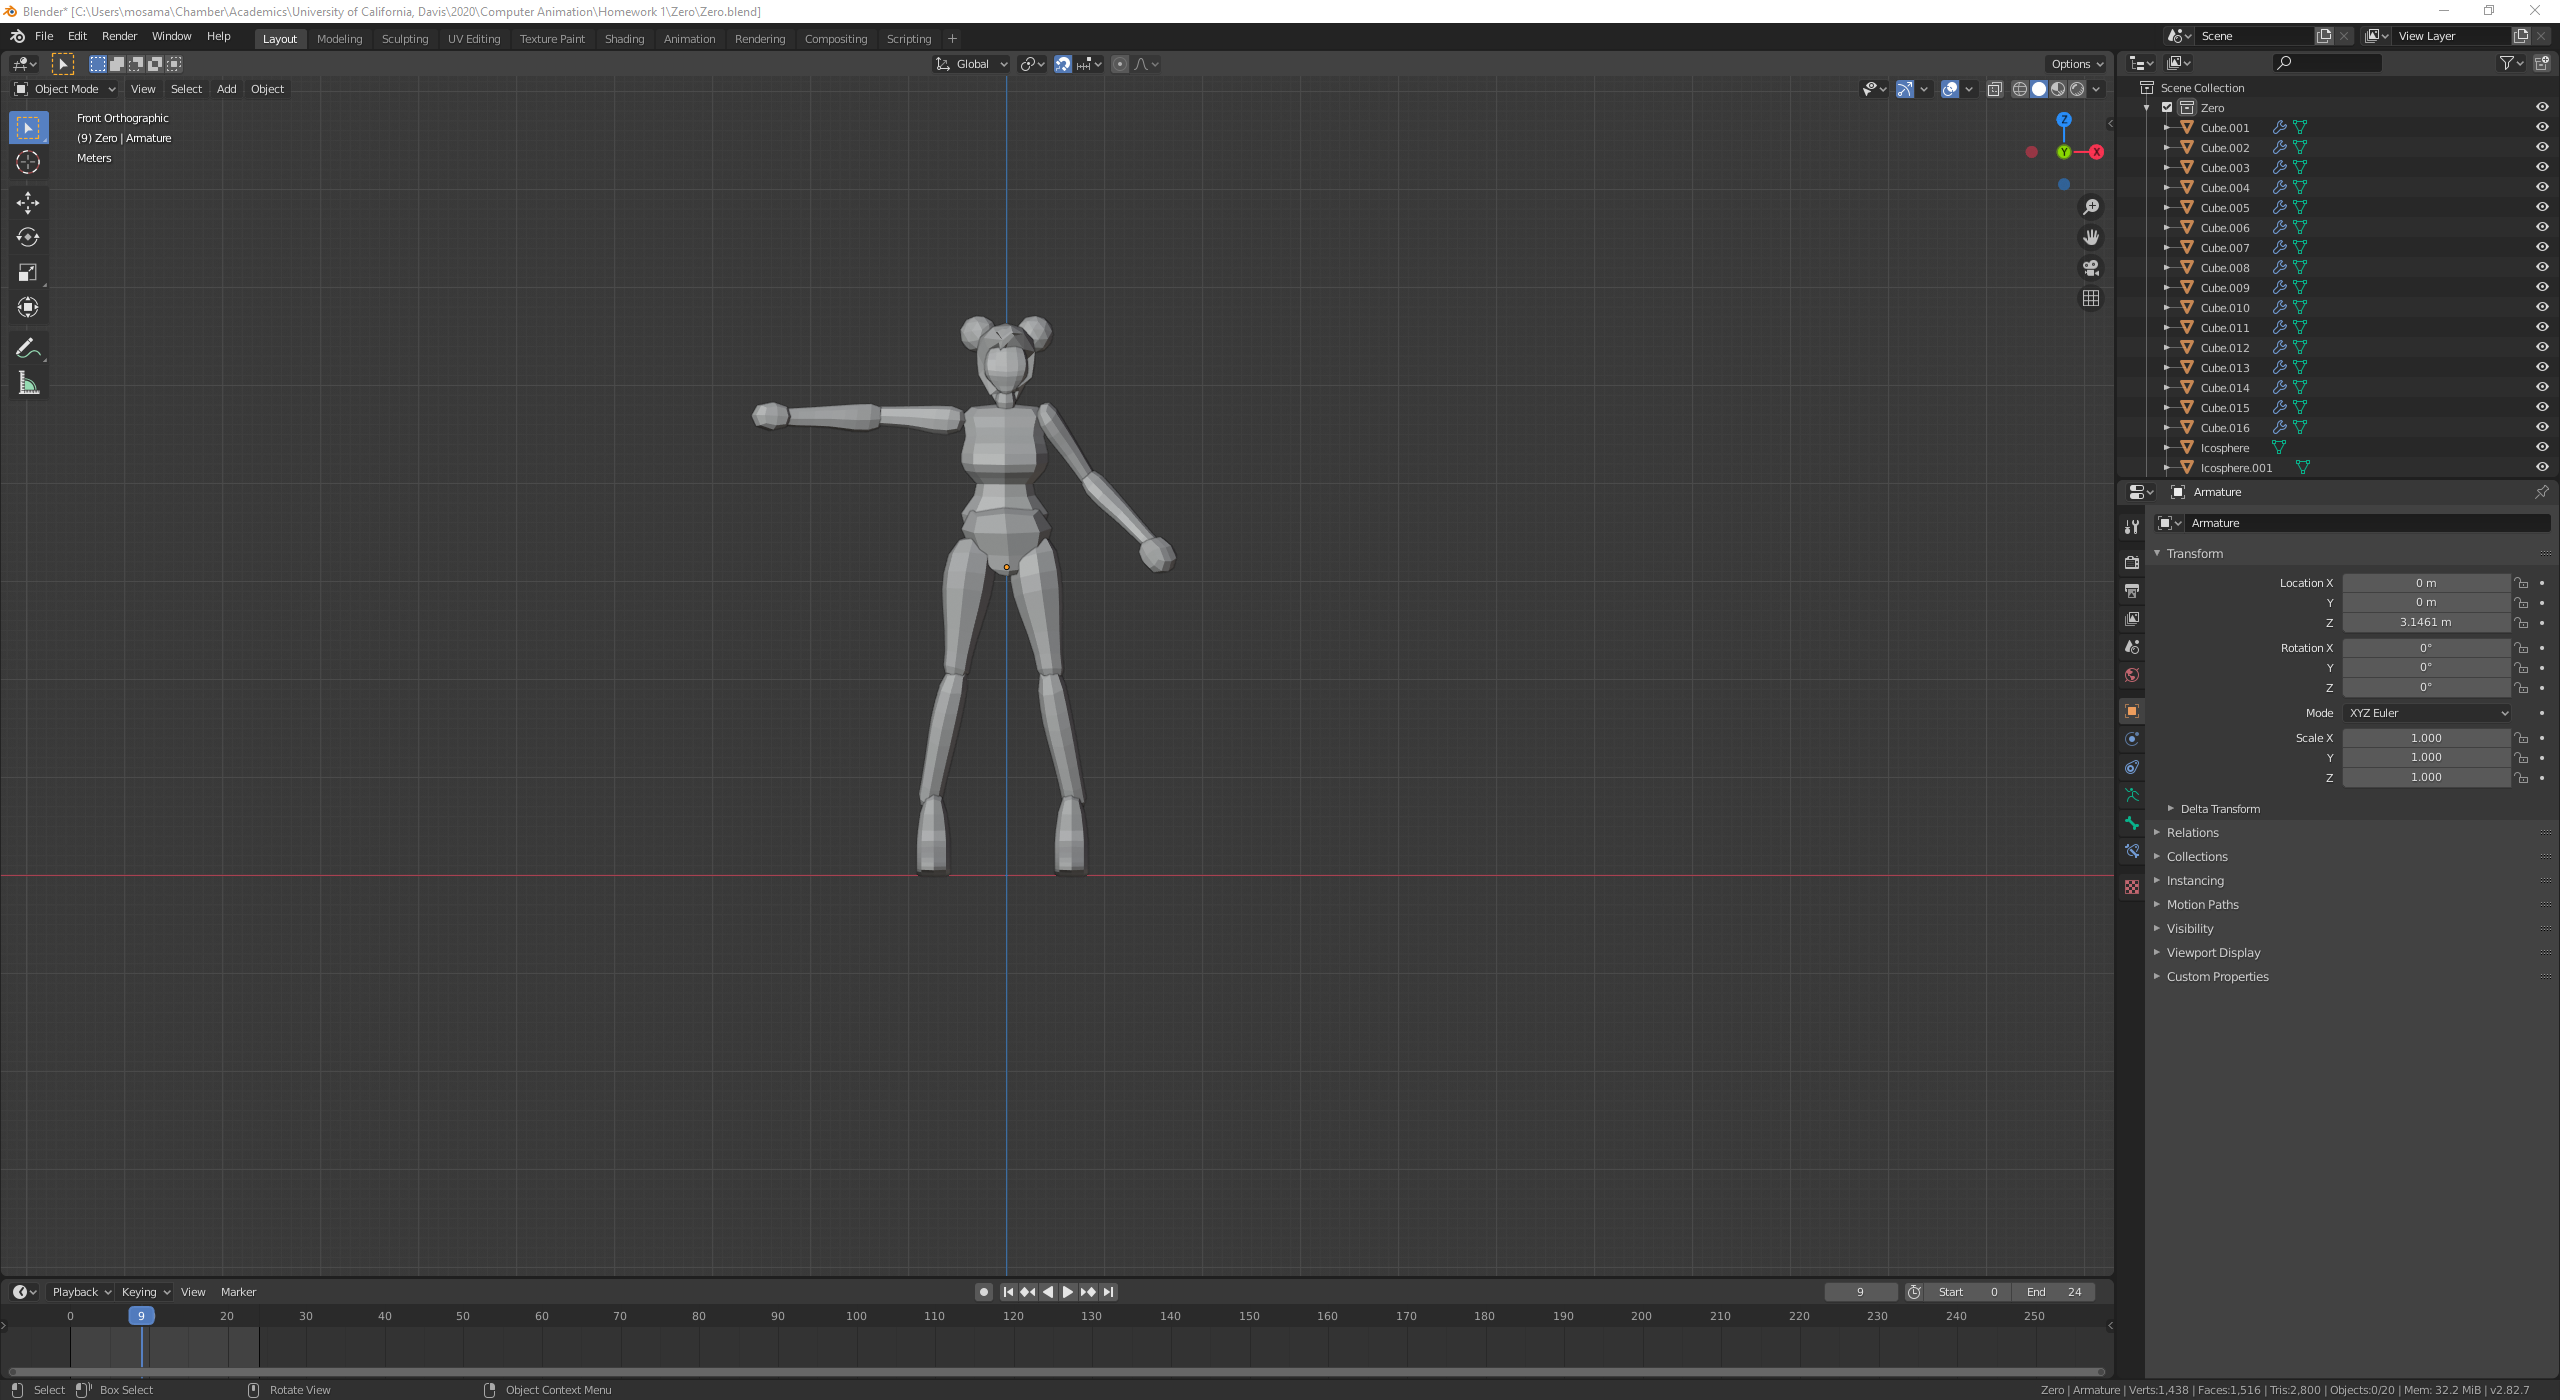
\includegraphics[width=0.23\textwidth]{images/Model_Front.png}
  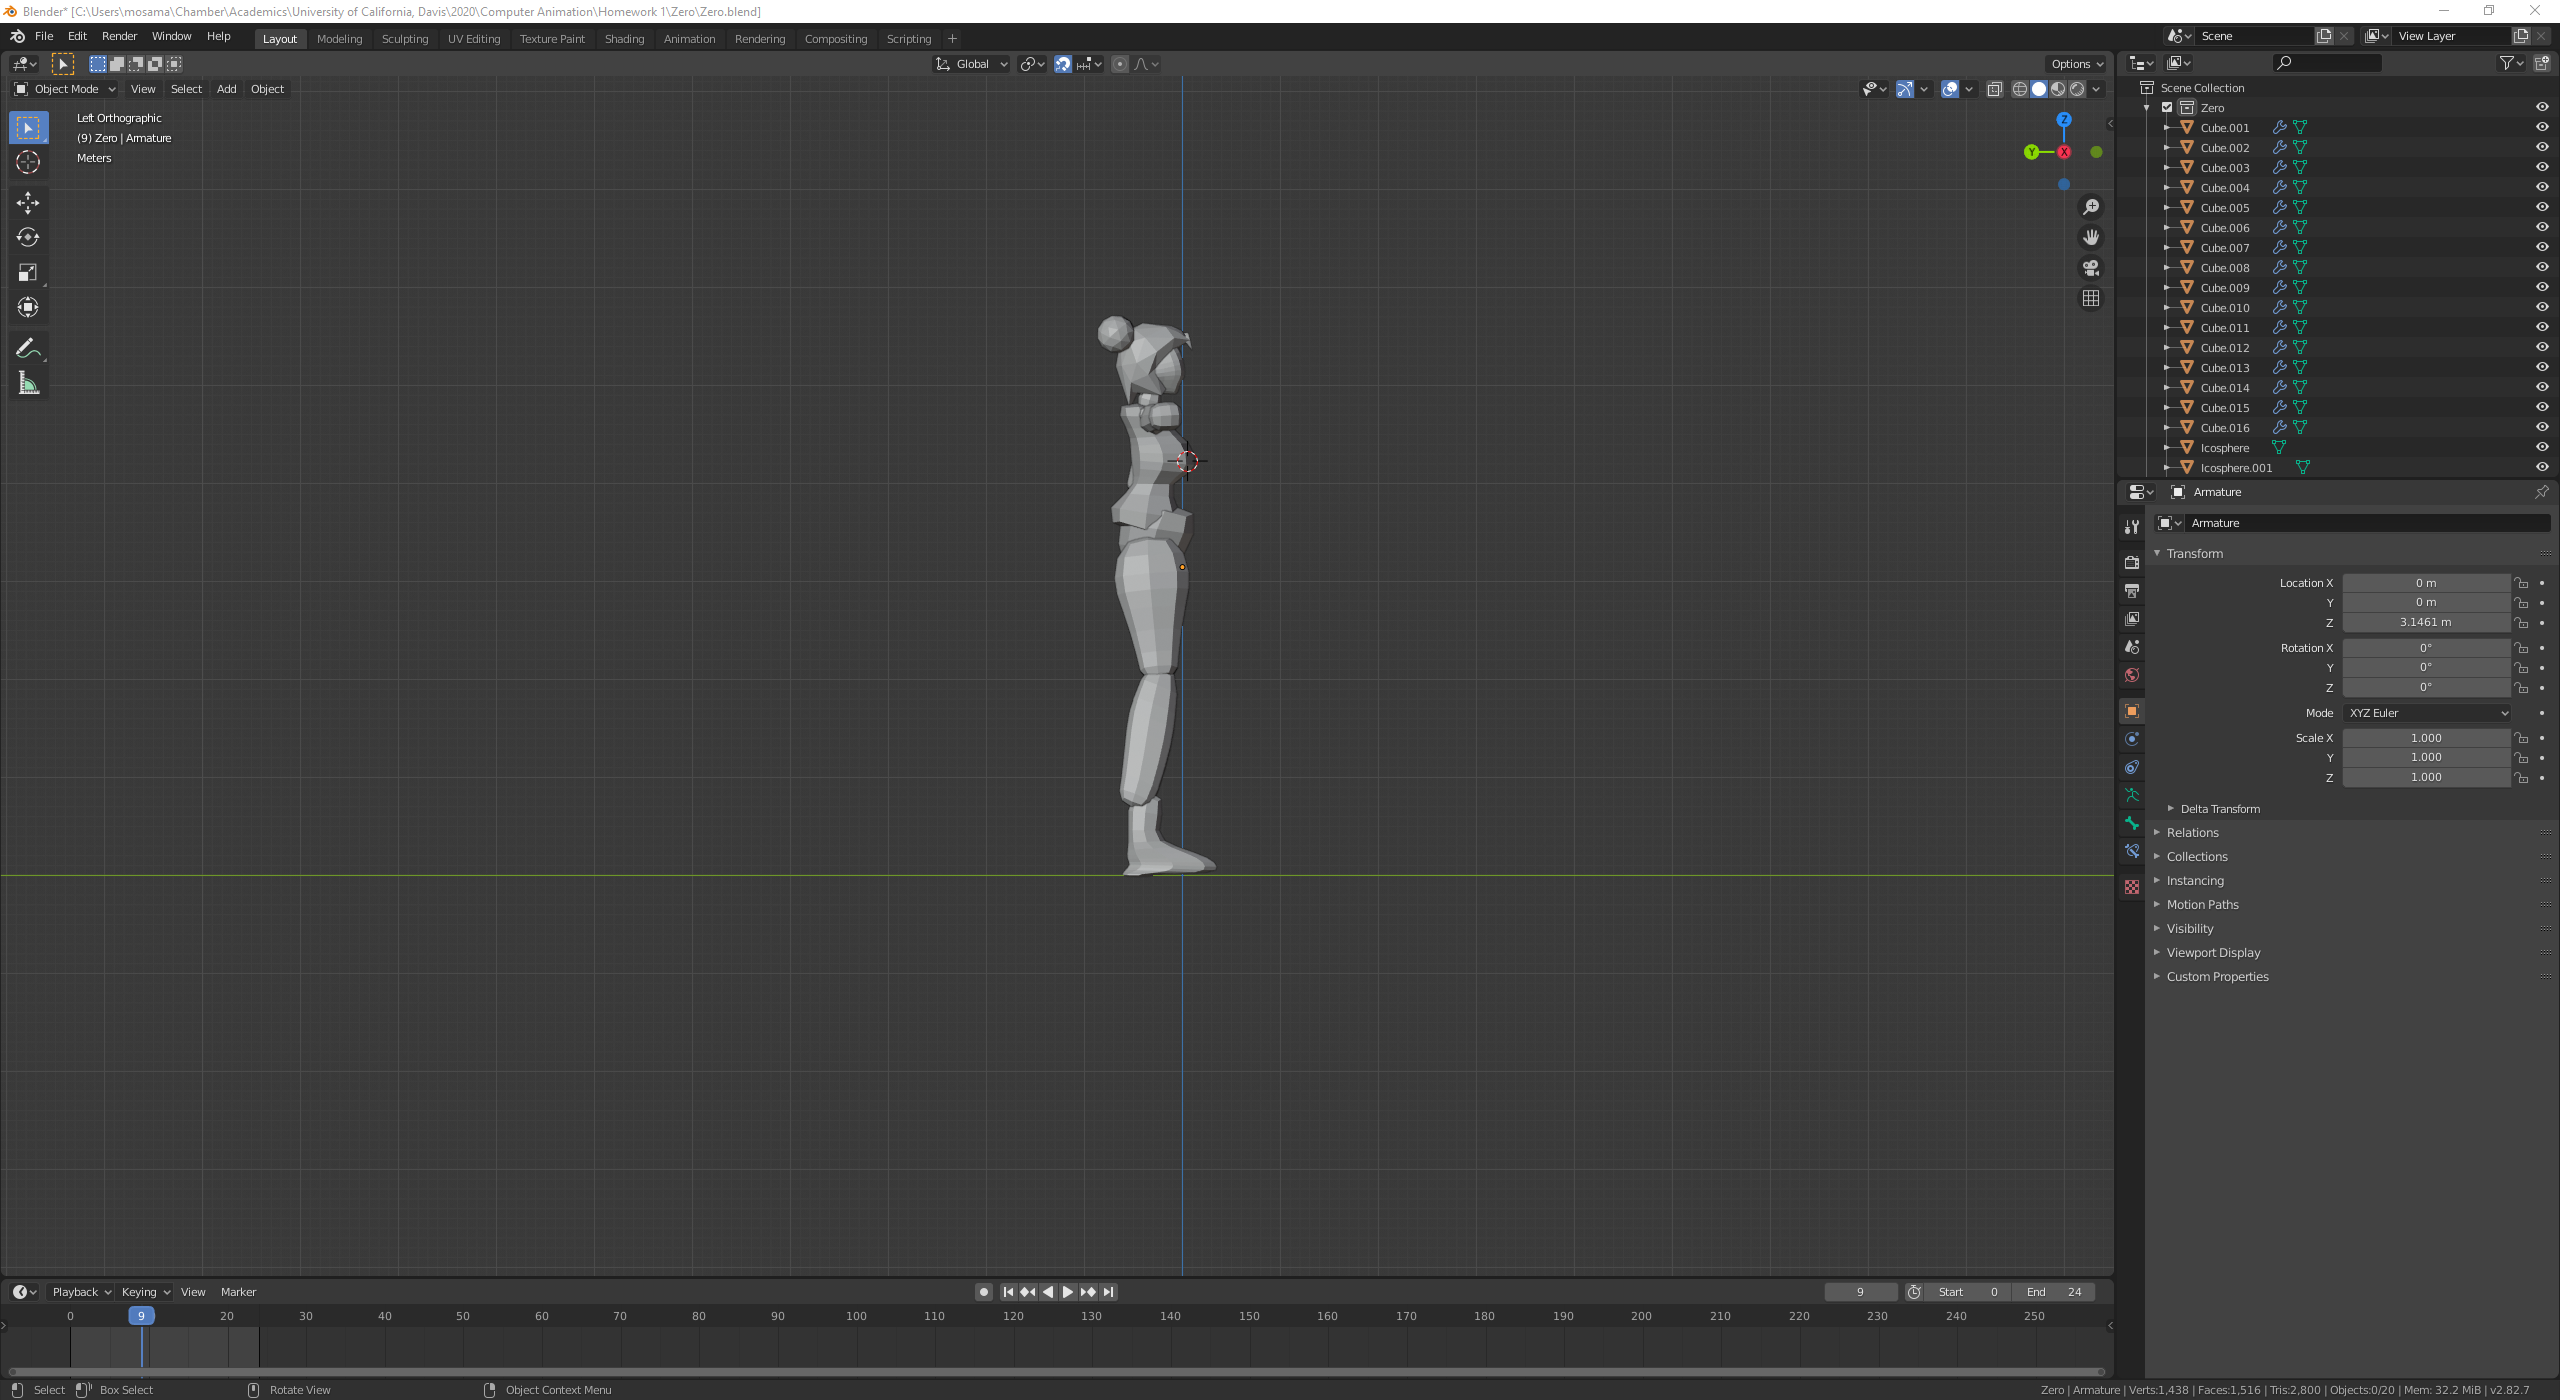
\includegraphics[width=0.23\textwidth]{images/Model_Side.png}
  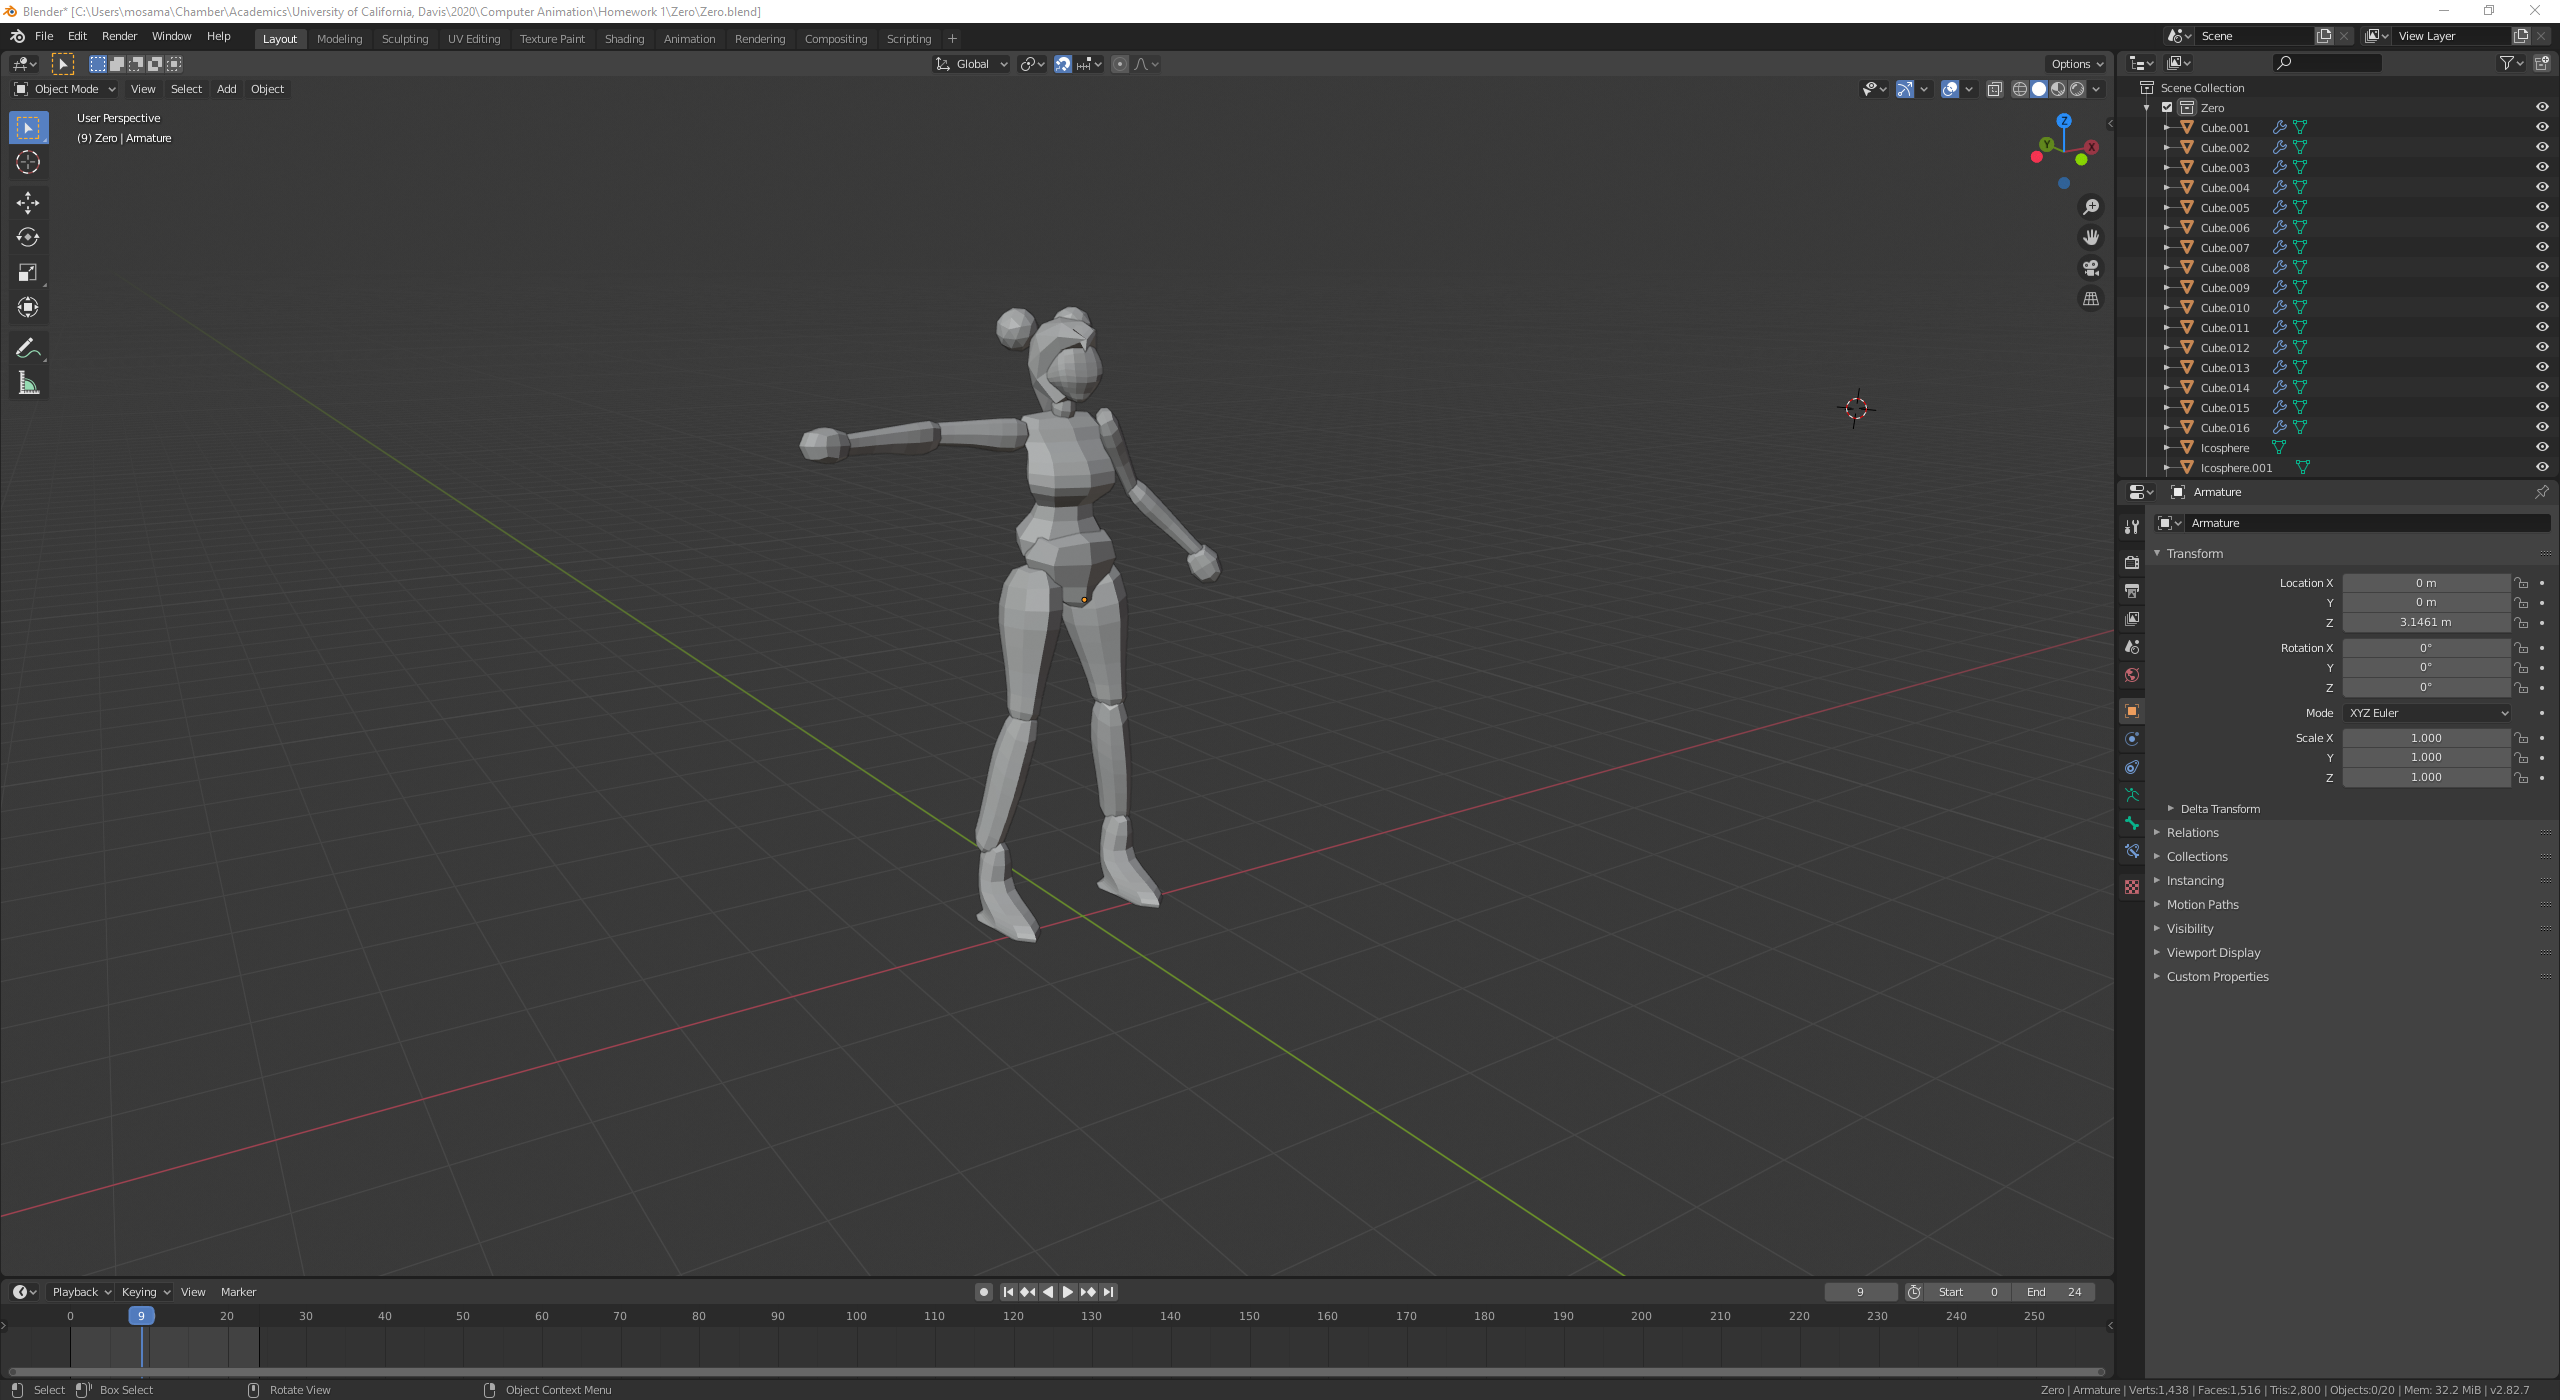
\includegraphics[width=0.47\textwidth]{images/Model_3D.png}
  \caption{Figures above show the front, side and 3D view of the model created within Blender.}  \label{fig:model}
\end{figure}


\subsection{Rigging a Model}
Once again for rigging, I used Blender and another tutorial by Grant Abbitt\cite{Blender:Rigging:Tutorial} on Rigging. Rigging process was a bit tedious, I added bones to every limb I created within my humanoid and named it accordingly. One lesson I learned after the fact was that I could've used replication/duplication and only modeled and rigged half of the model and just duplicated it to the other half to achieve symmetry. But since I had already gone ahead and rigged the whole thing manually, I chose to stick with it  for this project.

\subsection{Animating a Model \& Inverse Kinematics}
The most challenging part within animation was in-fact implementing Inverse Kinematics (IK) to the bones. My initial attempt was using Blender's "Auto IK" feature, which automatically figures out the appropriate IK settings for a given model and adds them accordingly. But to be able to actually add animated sequences and poses, I had to stray away from the Auto IK and manually implement it myself. I soon realized while adding IK constraints to each bone was that I needed more than just the bones of the skeleton to avoid problems such as singularity and odd motions. I added target and controller bones \textit{outside} the mesh of the humanoid and set those as the target and controller constraints within my IK implementation. With that, I added IK to arms, legs and torso, with copy rotation constraints on the head and hands matching the controller. This made for an interesting structure which I could then manipulate for more complicated animations such as walking. 

\begin{figure}[ht]
  \centering
  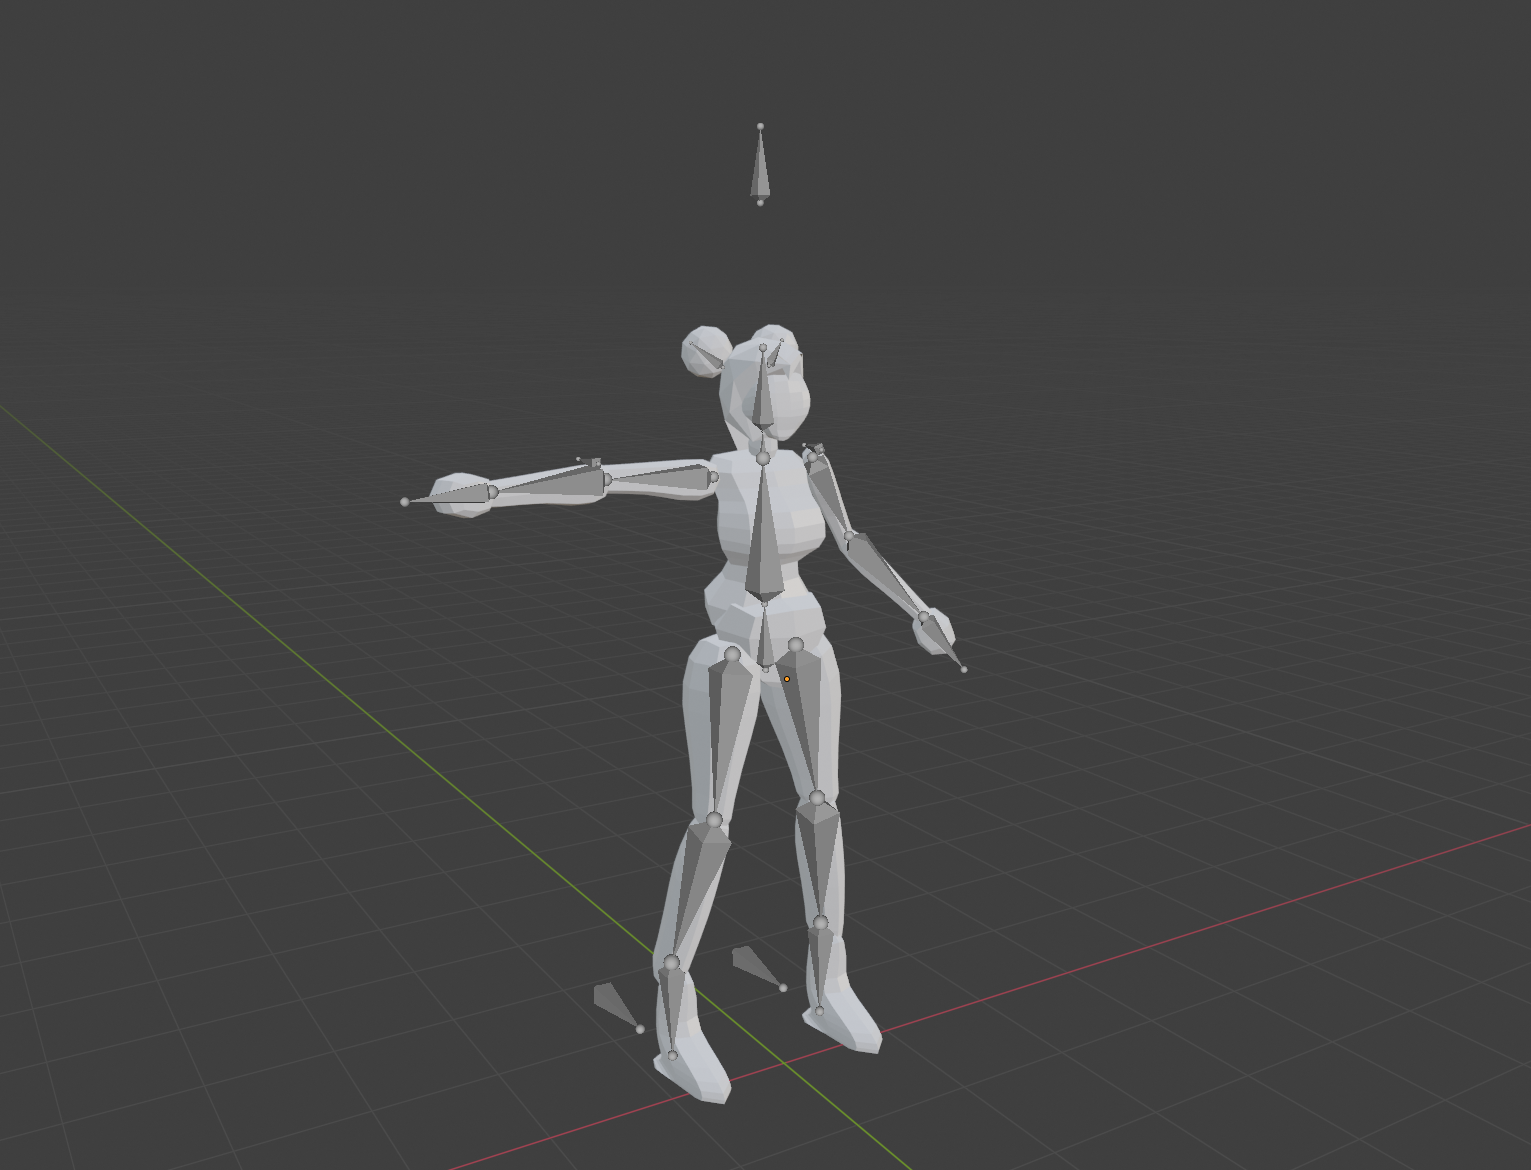
\includegraphics[width=0.47\textwidth]{images/rigged.png}
  \caption{Figures above show the 3D view of the rigged bones structure along with the controller and target bones for neck, hands and feet.}  \label{fig:rigged}
\end{figure}

\subsubsection{Inverse Kinematics (IK)}
Inverse Kinematics is essentially movement of bones/joins such that when the end point of a structure is moved (for example hands), the entire structure adjusts accordingly to reach a target position (structure being arms and shoulder in this example). IK within the bones uses a \textbf{Jacobian pseudoinverse}, which is essentially considering a small change in the join position and rotation that eventually leads to a state where position is equal to the end-effector. If joint configuration change is defined by $\delta q$, and we want the end-effector to move from position $x$ to $x_d$, $q_{next} = q + \alpha J^{+} (x_d - x(q))$, where $J^{+} = J^T (JJ^T)^{-1}$.

I implemented a 24 frames walking sequence. I used yet another reference image for this and keyed frames for different walking poses. And manually added the key frames for each of the steps. My model's movement was 4 frames a part and made for a semi-realistic walking simulation. Figure~\ref{fig:walking} shows the Blender timeline and keyframes for the walking animation of my model.

\begin{figure}[ht]
  \centering
  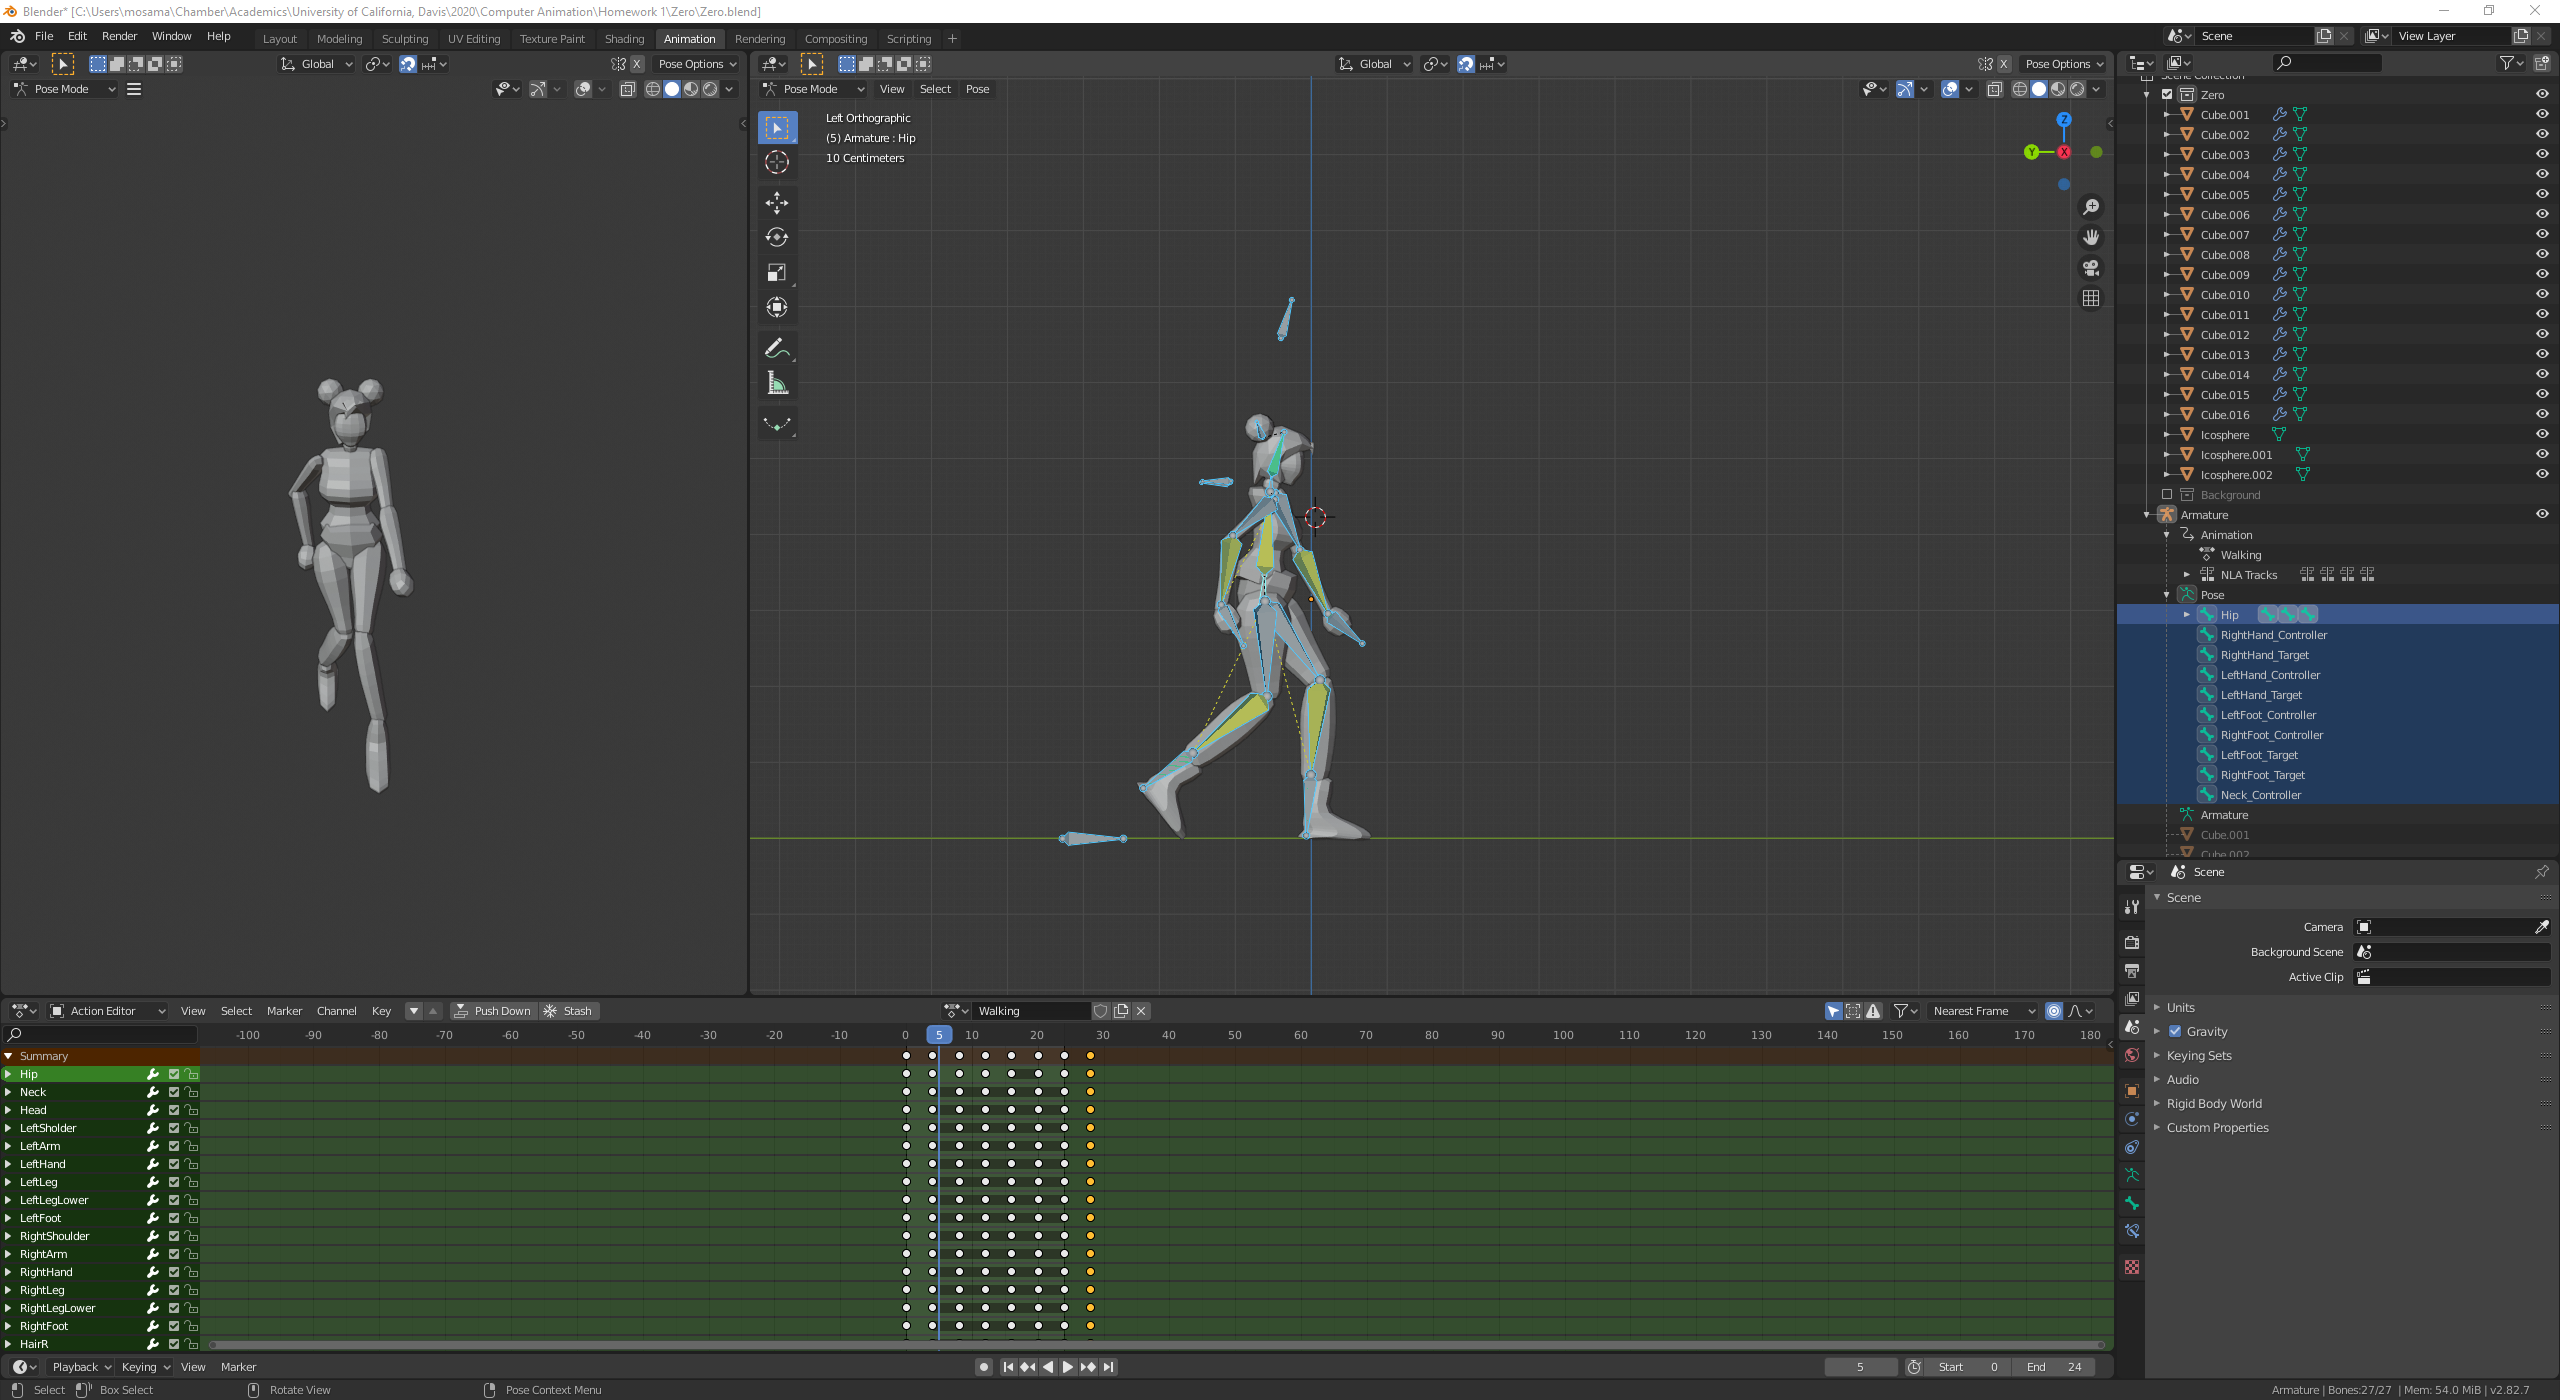
\includegraphics[width=0.47\textwidth]{images/walking.png}
  \caption{Shows the keyframes and a single frame of both 2D and 3D view of the 24FPS walking animation.}  \label{fig:walking}
\end{figure}

\section{Unreal Engine 4}
I managed to successfully import the model into Unreal Engine 4, but whenever I tried working on it my UE4 crashed with an error of Illegal Memory Access at index 0 for Array core file, which turned out to be a bug in UE4. I had a scene set up in UE4 where I have a top-down 3D environment and I can click a button to spawn trees, therefore, constructing an "ecosystem". But due to the crash, right now, I am only able to use the existing model and not the new animated one I created. (I have included both projects in the submission).


\bibliography{main.bib}
\bibliographystyle{ieeetr}

\end{document}
